\chapter{}{Multi-Model Approach to Solar Irradiance Forecasting}

\subchapter{Overview}
For days-ahead forecast horizon, regional and global numerical weather prediction models, predicting the evolution of the atmospheric system have been shown to be more appropriate and accurate \cite{thesis_zach}. The numerical weather prediction models derive their initial conditions from different ground and airborne sensors from across the world. Based on thermodynamic equations describing the physical processes occurring in atmosphere, they forecast different weather variables into the forecast horizon. The National Oceanic and Atmospheric Administration (NOAA) operates a variety of numerical weather prediction models with their spatial resolution ranging from approximately 10 km - 50 km, and their temporal resolution typically being 1 hour or 3 hours -  which are normally updated every 6 hours \cite{multimodel_bestpractices}. 

\par In this work, we intended to forecast solar irradiance captured at the solar farm in Athens, Georgia for a forecast horizon of 24 hours. For this purpose, a mesoscale model such as the \textit{North American Mesoscale (NAM)} Forecast System \cite{multimodel_nam} which can predict parameters describing cloudiness was used. Typical weather variables known to affect solar irradiance forecasting systems such as air temperature, geopotential height, cloud cover, visibility, wind speed, dew point temperature, air pressure, downwelling shortwave radiation flux, downwelling longwave radiation flux, and humidity were evaluated so as to gauge their effect on the solar irradiance predictions. It was observed that the irradiance readings from the solar farm for each of the arrays were influenced more by the surface temperature, downwelling short-wave radiation flux, total cloud cover, and atmospheric height. Thus, the remaining weather variables were discarded. This enabled a cut in computational cost of modeling and also led to an improvement in the performance of the models.

\restoregeometry

\par Downwelling shortwave radiation flux, synonymous with global horizontal irradiance (GHI) is measured by NWP models using columnar radiative transfer models (RTM). The RTMs help in determining cloud optical properties for different wavelength bands with the help of weather variables such as air temperature, gas concentrations and cloud structure. Thus, they contribute to effective cloud modeling, and in turn, effective shortwave radiation flux computation. However, the direct output from the mesoscale models has shown severe deviations between forecasted and real irradiance \cite{multimodel_ghi}. While the usage of additional weather variables in machine learning models have shown to improve the post-processing of NWP models by incorporating site-specific information, it has to be taken into consideration is that there is a significant variability in the GHI measured by the NWP models with respect to the cloud conditions. As a matter of fact, Mathiesan et al \cite{multimodel_overpredict} found that the NAM forecast model tends to overpredict GHI in clear-sky conditions (absence of visible clouds) by up to 40 percent. Thus, a need was identified to correct the bias in the GHI measured by the NAM Forecast System, specifically in the clear-sky conditions.

\par There are multiple formulations which have been extensively discussed in literature, which compute the irradiance metrics from environmental conditions such as cloud cover. These can be broadly classified into decomposition models and isotropic models. Using assumptions on solar geometry and transmittance, the former are used to estimate direct beam and diffuse irradiance. The latter are useful for approximating daily solar radiation reaching tilted surfaces. GHI can be empirically estimated from these irradiance metrics. The GHI thus estimated can be used to further correct the bias in GHI forecasts recorded by the NWP models.

\subsubchapter{Numerical Weather Prediction (NWP) Models}
Solar forecasting researchers have successfully employed meteorological forecasts from Numerical Weather Prediction (NWP) models for forecasting applications for years. The making of a weather forecast involves assessing the current weather situation, assimilating observational information, and projecting this initial state into future based on the laws of thermodynamics. Weather forecasting employs a set of equations that describe the flow of fluids, being run over a geographic area. Several parameterizations of physical processes are carried out, based on the physical and statistical representations of the physical process. This is useful to approximate the bulk effects of the physical processes.

\par One of the major challenges faced in this process is determining the range of area to observe. As shown in Fig.~\ref{fig:fig_variability}, the further the forecasting of the weather conditions, i.e, higher the forecast horizon, wider is the range of area that needs to be observed. Multiple weather prediction models, both global and regional, depending on the spatial domain, are maintained by the National Oceanic and Atmospheric Administration (NOAA). Global Forecast System (GFS) is one of the widely-known global weather prediction models, which represents the atmospheric state as a superposition of wave functions. It covers the entire globe at a base horizontal resolution of $28km$ between grid points, predicting weather out to $16$ days. Within continental United States, North America Mesoscale (NAM), Rapid Refresh (RAP), High Resolution Rapid Refresh (HRRR) are the popular regional weather prediction models, each having it's own advantages. The NAM model follows a complex cloud prediction scheme accounting for the internal cloud processes, and thus has better cloud parameterizations over RAP and HRRR. Thus for our experiments, we chose the NAM model data and created a weather forecast dataset spanning the years 2017 and 2018, though a few forecasts are missing sporadically.

\begin{figure}[ht]
    \begin{center}
    	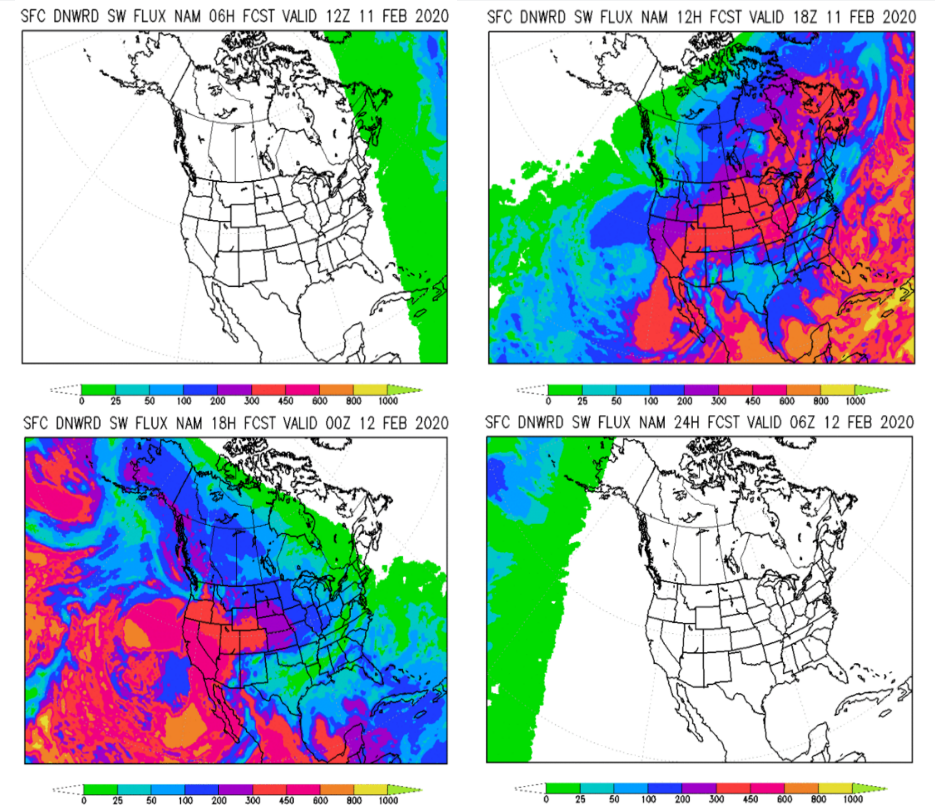
\includegraphics[width=0.85\textwidth]{chapter3/fig_nam_dswrf.png}
    	\caption[Downward shortwave radiation flux parameter for 06h, 12h, 18h, 24h UTC forecasts in a day for NAM model data]{Downward Shortwave Radiation Flux parameter from NAM data over North America domain for 06h forecast (top-left), 12h forecast (top-right), 18h forecast (bottom-left) and 24h forecast (bottom-right) UTC for 11th February, 2020.}
    	\label{fig:fig_nam_dswrf}
    \end{center}
\end{figure}

\par The NAM Forecast System is based on the Weather Research and Forecasting (WRF) model infrastructure, following non-hydrostatic dynamics and thus enabling vertical momentum estimations. It provides high resolution forecasts over North America for a forecast horizon of 84 hours, the first 36 of which are at a one hour temporal resolution, and the remaining thereafter, at a 3 hour temporal resolution. The forecasts are published for a grid spanning approximately $12km$ x $12 km$ across the continental United States, which are released four times daily at 00h, 06h, 12h and 18h UTC.

\par Following the update in 2017, the current version of the NAM model follows Janjic-modified Betts-Miller convection \cite{multimodel_janjic} for parameterization of physical processes, RTM-based longwave and shortwave prediction scheme, and an updated Ferrier-Aligo predictive cloud scheme \cite{multimodel_cloud}. The NWP models cannot resolve weather features and physical processes that occur within a single grid box. Vertical redistribution of heat and moisture can easily occur between mesoscale grids resulting in sub grid-scale variations in convection. The Janjic-modified Betts-Miller convection scheme nudges the temperature and moisture profiles in a grid towards a specific reference profile through repeated observations, thus improving the convection parameterizations in the NAM model by decreasing the convective instability.

\par For convective time scales of the order of 30 minutes to 1 hour, radiative heating rates are negligible. However, for the NAM data which has a forecast length of 84 hours, radiative transfer processes in the clouds need to be taken into consideration as well. In a cloud-free atmosphere, the primary absorbers of shortwave radiation are ozone and water vapour. However, in a cloudy atmosphere, shortwave radiation is more complicated, and a spectrum of radiative frequencies on cloud absorption, reflection and transmission need to be considered \cite{multimodel_rtm}. The NAM models implement the columnar RTM models in this effect, which for each vertical level parameterize the cloud radiative properties.

\par Dozens of parameters are available in a NAM model data grid pertaining to environmental components such as altitude, atmospheric pressure, atmospheric radiation, air temperature, water vapour, atmospheric winds, precipitation, soil properties and cloud cover. The features are spread across 60 vertical levels in a 0 - 3 km layer, and across 39 pressure levels from 50mb to 1000mb at 25mb intervals. From among these parameters, in Fig.~\ref{fig:fig_nam_dswrf}\footnote{NAM forecast snapshots retrieved from: \url{https://www.emc.ncep.noaa.gov/mmb/mmbpll/etapll}}, the averaged downwelling short-wave radiation flux over North America for the four forecasts on 11th February, 2020 is reported.

\subsubchapter{PVLIB Forecast Modeling}
Holmgrem et al \cite{pvlib_Holmgren2018} contributed to building \textit{pvlib-python}\footnote{\url{https://github.com/pvlib/pvlib-python}} an open source, python-based tool, ported from the PVLIB MATLAB toolbox developed at Sandia National Laboratories. This software provides a set of utilities for simulating the performance of the photovoltaic energy systems, with implementations of algorithms related to solar energy. Specifically, it contains components to obtain weather forecast data from NOAA/NCEP/NWS models including the GFS, NAM, RAP, HRRR, and the NDFD, retrieved from the UNIDATA THREDDS servers; and components to convert this weather forecast data into a PV power forecast. 

\par For our experiments, we created a NAM weather forecast dataset for the years of 2017 and 2018, retrieved from the NCEP servers. Meanwhile, \textit{pvlib-python} retrieves NAM CONUS 12km resolution forecasts from the THREDDS servers. The key difference between each of these NAM products is that the former is a full complement of both the pressure level fields and surface-based fields, while the latter is a full complement of just the surface-based fields. The NAM data retrieved and processed by \textit{pvlib-python} consists of the following parameters: air temperature, wind speed, total clouds, low clouds, mid clouds and high clouds. In order to be able to use the \textit{pvlib-python} functionalities on the weather forecast dataset collected by us, equivalent surface-level fields were identified in our weather forecast dataset. Thus, compatibility between the NAM data obtained from both the sources was established, enabling the use of \textit{pvlib-python} functionalities on this engineered dataset.

\par \textit{pvlib-python} software contains components, which are implementations of several theoretical formulations to compute irradiance metrics such as diffuse horizontal irradiance (DHI), direct normal irradiance (DNI) and global horizontal irradiance (GHI) from the weather forecast data. DHI is the amount of solar radiation received by a horizontal surface, which has been scattered by the molecules and particles in the atmosphere. It is the part of the solar radiation which does not belong to the $5^{\circ}$ field of view concentric around the sun, and is typically measured with a pyranometer. DNI is the direct radiation received on a plane normal to the sun over the total solar spectrum. It is an essential component of global irradiance, especially in cloudless conditions, and can be measured with the help of a pyrheliometer. While the solar radiation incident on the earth's atmosphere is relatively constant, various factors such as atmospheric conditions, latitude of the location, season of the year, etc. affect the amount of solar radiation incident on the earth's surface. GHI is the total amount of such terrestrial irradiance which is received by a surface horizontal to the surface of the earth. It can measured with the help of pyranometers, and in general, can be computed from DHI and DNI using the following equation, where $\theta_z$ is the \textit{zenith angle} (the angle between sun and the vertical):
\begin{equation}\label{eq:ghi}
    GHI = DHI + DNI . cos(\theta_z)
\end{equation}

\par Each of these irradiance metrics were computed from the \textit{pvlib-python} compatible dataset using two empirical techniques implemented in the software: Clearsky Scaling, Liu Jordan.


\subsubsection*{Clear-sky Scaling}
\par Global horizontal irradiance can be measured with the help of a pyranometer on a horizontal surface, and thus, is typically the most common type of irradiance measurement. Knowledge of the clear sky conditions (absence of visible clouds), is a key requirement for forecasting all three irradiance metrics. Clear-sky models estimate the terrestrial solar radiation under a cloudless sky from various atmospheric conditions. Such models can be generally validated by comparing the measured irradiance in the clear-sky conditions. 

\par Several parametric models have been proposed in literature to compute these irradiance metrics from environmental conditions such as atmospheric turbidity, fractional sunshine, perceptible water vapor, etc. Ineichen et al \cite{pvlib_ineichen} formulated a model to compute Linke turbidity independent of the airmass, and clear-sky GHI from this metric. Going by Larson et al's \cite{pvlib_larson} work, \textit{pvlib-python} scales global horizontal irradiance on the basis of the total cloud cover and clear-sky GHI according to the following equation, where $GHI_{CS}$ is the clear-sky GHI and TCC is the total cloud cover:
\begin{equation}\label{eq:ghi_cs}
    GHI = GHI_{CS} . [0.35 + 0.65(1 - TCC)]
\end{equation}

\par Maxwell et al \cite{pvlib_disc} introduced the popular \textit{Direct Insolation Simulation Code} (DISC) model to compute cloudy-sky DNI from GHI (in this case, computed with Eq. \ref{eq:ghi_cs}) and other environmental factors. Clearness index is the fraction of the solar radiation transmitted through the atmosphere to strike the earth's surface. DISC model uses empirical relationships between the direct and global components of this measure to estimate the direct beam component. Additionally, the clear-sky DHI component can be evaluated from these irradiance metrics and the solar zenith angle using the equation described in Eq. \ref{eq:ghi}.


\subsubsection*{Liu-Jordan Method}
Decomposition models typically utilize only data pertaining to global radiation to estimate diffuse radiation from global solar irradiation data, as can be seen in the previous subsection. They are based on the atmospheric effects in an isolated place, varying according to time of the year, season and climatic conditions \cite{pvlib_liujordan}. Liu et al proposed one of the earliest and simplest models of radiation, the Liu-Jordan model \cite{pvlib_liujordan2}, which presumes that diffuse radiation intensity is distributed uniformly over the whole sky, and helps estimate diffuse radiation on inclined surfaces. In this model, the diffuse irradiance on a surface tilted towards the equator at an angle $\theta$, where $I_D$ is the diffuse radiation on a horizontal surface is given by the following empirical equation:
\begin{equation}\label{eq:lj_dhi}
    I_{Dt} = I_D . (\frac{1 + cos\theta}{2})
\end{equation}

Liu-Jordan model, though simple, is one of the more accurate among isotropic models for estimating diffuse radiation on inclined surfaces \cite{pvlib_liujordan3}. This model helps determine direct normal irradiance, global horizontal irradiance from properties such as extraterrestrial flux, transmittance, and optical air mass number. It has been observed that the Liu-Jordan model provides a good fit to empirical data under overcast skies, but underestimates the solar radiation on tilted surfaces when used for partially-clear and clear-sky days \cite{pvlib_liujordan4}.

\subchapter{Data Collection and Pre-processing}
\subsubsection*{Weather Forecasts}
\begin{table}[h]
\begin{center}
    \caption{NWP-NAM variables retrieved for solar forecasting}
    \label{Tab:table_nam_variables}
    \begin{tabular}{ c c c}
    	\toprule
    	\textbf{Label} & \textbf{Description} & \textbf{Unit} \\
    	\midrule
    	PRES\_SFC & Air Pressure & $Pa$\\
    	HGT\_SFC & Geopotential Height & $gpm$ \\
    	HGT\_TOA & Height at Planetary Boundary Layer & $gpm$ \\
    	TMP\_SFC & Air Temperature & $K$\\
    	VIS\_SFC & Visibility & $m$\\
    	UGRD\_TOA & U-Component of Wind Speed & $m/s$\\
    	VGRD\_TOA & V-Component of Wind Speed & $m/s$\\
    	DSWRF\_SFC & Downward Short-Wave Radiation Flux & $W/m^2$\\
    	DLWRF\_SFC & Downward Long-Wave Radiation Flux & $W/m^2$\\
    	TCC\_EATM & Total Cloud Cover & $\%$ \\
    	\bottomrule
    \end{tabular}
\end{center}
\end{table}

\par As mentioned in 3.1.1, North America Mesoscale (NAM) model data was collected from the years 2017 and 2018 for experiments. From this data, surface-level parameters as described in Table \ref{Tab:table_nam_variables} were retrieved and analyzed. NAM model projects different weather parameters 84 hours into the future, the first 36 hours of the forecast horizon at a 1-hour temporal resolution, and subsequent 48 hours of the forecast horizon at a 3-hour temporal resolution. In this work, we consider the first 24 hour projections of each of the weather parameters along with their corresponding target pyranometer readings.

\subsubsection*{Temporal Features}
\par In \cite{thesis_zach}, Jones et al. extracted temporal features by parameterizing the \textit{time of day} and \textit{time of year} of the forecasts. These measures were computed by scaling the epoch representing the reference time (in nanoseconds) with the inverse of $8.64e+13$ (number of nanoseconds in a day) and $3.1536e+16$ (number of nanoseconds in a year) respectively. The sine and cosine values of these measures were included, resulting in four temporal features, two each representing the \textit{time of day} and \textit{time of year}. However, this approach fails to capture the cyclicity of the reference time in a particular day, or that of a day in a particular month, in a year. In this work, these parameterizations  were modified to represent the hour in a day and the day in a month respectively. The \textit{time of day} was computed by scaling the number of seconds in the reference time with the inverse of $8.64e+4$ (number of seconds in a day); and the \textit{time of year} was computed by scaling the day of the year with the inverse of $365$ or $366$, depending on whether it is a leap year or not. The sine and cosine values of these measures were added as the temporal features. Additionally, such temporal features of the reference time representing the corresponding target hours were also included in their respective predictors.

\subsubsection*{Irradiance Observations}
\par Georgia Power, in collaboration with the University of Georgia set up a 1MW solar facility in Athens, Georgia. The irradiance observations are obtained from three solar arrays in the solar farm, namely array A, array B and array E, representing a dual-axis tracking array, fixed axis array with 200$^{\circ}$(SW) azimuth, and a single-axis tracking array respectively. Each of the solar arrays are installed with thermopile pyranometers from different manufacturers such as Kipp \& Zonen\footnote{\url{https://www.kippzonen.com/}}, and LICOR\footnote{\url{https://www.licor.com/}}. The thermopile pyranometers have a black absorptive surface which uniformly absorbs the solar radiation across the short-wave solar spectrum, i.e, between 0.2 $\mu m$ and 3 $\mu m$. 

\begin{figure}[ht]
    \begin{center}
    	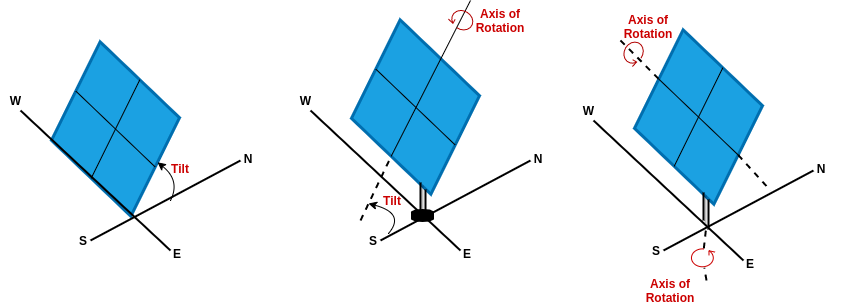
\includegraphics[width=0.85\textwidth]{chapter3/fig_pyranometers.png}
    	\caption[Fixed axis, Single-axis tracking, Dual-axis tracking Solar Arrays]{Fixed axis (left), Single-axis tracking (center), Dual-axis tracking (right) Solar Arrays.}
    	\label{fig:fig_pyranometers}
    \end{center}
\end{figure}

The fixed axis solar array, i.e, array B has limited exposure to the sun, owing to the change in position of the sun during the day from morning to night. Thus, the solar radiation captured by array B is reduced. Though this limitation is negated by installing the fixed solar array at an optimized tilt angle, the solar radiation captured by solar tracking arrays is still considerably higher. In order to maximize the overall solar energy captured, it is necessary to ensure that the angle of incidence of the sunlight on the solar array is constantly perpendicular. This is achieved with the help of single-axis trackers (horizontal and vertical), which have one degree of freedom acting as an axis of rotation; and dual-axis trackers which have two degrees of freedom acting as axes of rotation normal to one another \cite{irradiance_solartracker}. This ability to move along the axes enhances the morning and afternoon performance of the solar tracking systems.

\begin{figure}[ht]
    \begin{center}
    	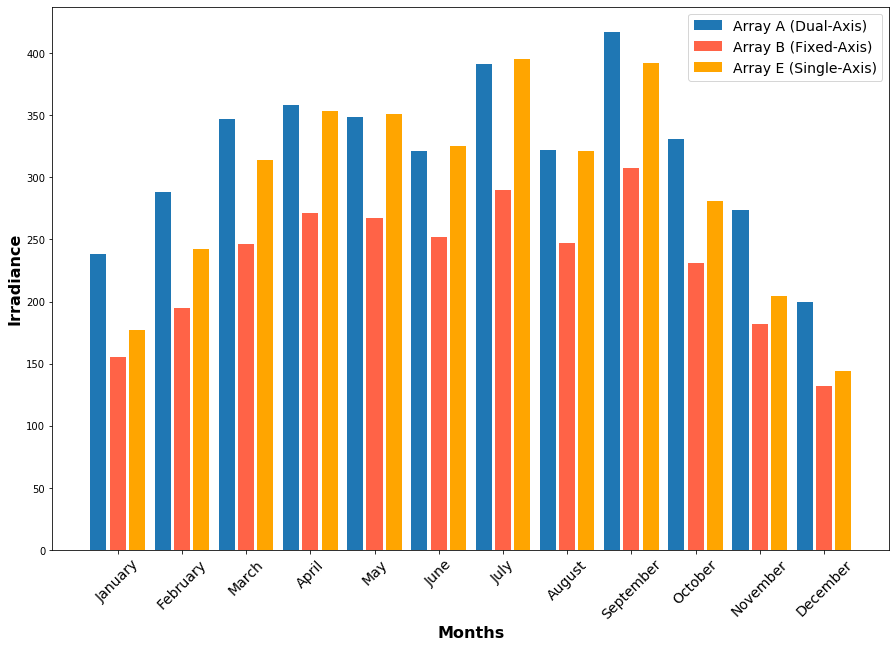
\includegraphics[width=0.85\textwidth]{chapter3/fig_average_irradiance.png}
    	\caption[Average monthly solar radiation captured by arrays A, B and E through 2017.]{Average monthly solar radiation captured by dual-axis (array A), fixed-axis (array B) and single-axis (array E) through 2017.}
    	\label{fig:fig_average_irradiance}
    \end{center}
\end{figure}

While the irradiance observations from the solar arrays are received every five seconds, the NWP NAM model data is available only for four reference times in a day, i.e 00h, 06h, 12h, 18h UTC through 2017 and 2018. Thus, for the target hours in the forecast horizon of all the reference times in 2017 and 2018, for which the NWP NAM model data was collected, the irradiance observations were sampled. In Fig.~\ref{fig:fig_average_irradiance}, the average monthly solar radiation captured by arrays A, B and E through 2017 is shown. It can be observed that the solar radiation captured by the tracking arrays, i.e, array A and array E is consistently higher than that captured by the fixed axis array, i.e array B.

\subsubsection*{Evaluating Impact of Weather Parameters on Irradiance Observations}
\par Mutual information is the measure between two possibly multi-dimensional variables, which quantifies the amount of information obtained from one variable about the other. The relationship detected between the variables can involve either mean, variance or even the higher moments \cite{feature_selection_mi}. The most straightforward and widespread approach towards estimating mutual information follows partitioning the supports of $X$ and $Y$ into bins of finite size, and approximating the sum in the following way:
\begin{equation}\label{eq:eq_mi}
I(X, Y) \approx I_{binned}(X, Y) \equiv \sum_{ij} p(i, j) . log(\frac{p(i, j)}{p_x(i).p_y(j)})
\end{equation}

In this work, the mutual information measure was estimated using the \textit{scikit-learn}\footnote{\url{https://scikit-learn.org/stable/}} machine learning software, which makes use of a non-parametric method based on entropy estimation from the k-nearest neighbors as described in \cite{feature_selection_mi} and \cite{feature_selection_mi2}. Mutual information measure was calculated for the different weather parameters from the NAM data and the irradiance observations from the solar arrays as described in the previous subsections. In Fig. \ref{fig:fig_mi_forecast_target_hr1}, mutual information between different NAM feature projections for the first forecast hour in the forecast horizon, and corresponding irradiance observations from array B is indicated, and their corresponding plots are shown. It can be observed that downward shortwave radiation flux (DSWRF\_SFC), air temperature (TMP\_SFC), height at planetary boundary layer (HGT\_TOA) and total cloud cover (TCC\_EATM) have a mutual information score greater than 0.1, indicating a higher dependency on the irradiance observations. 

\begin{figure}[htbp]
    \begin{center}
    	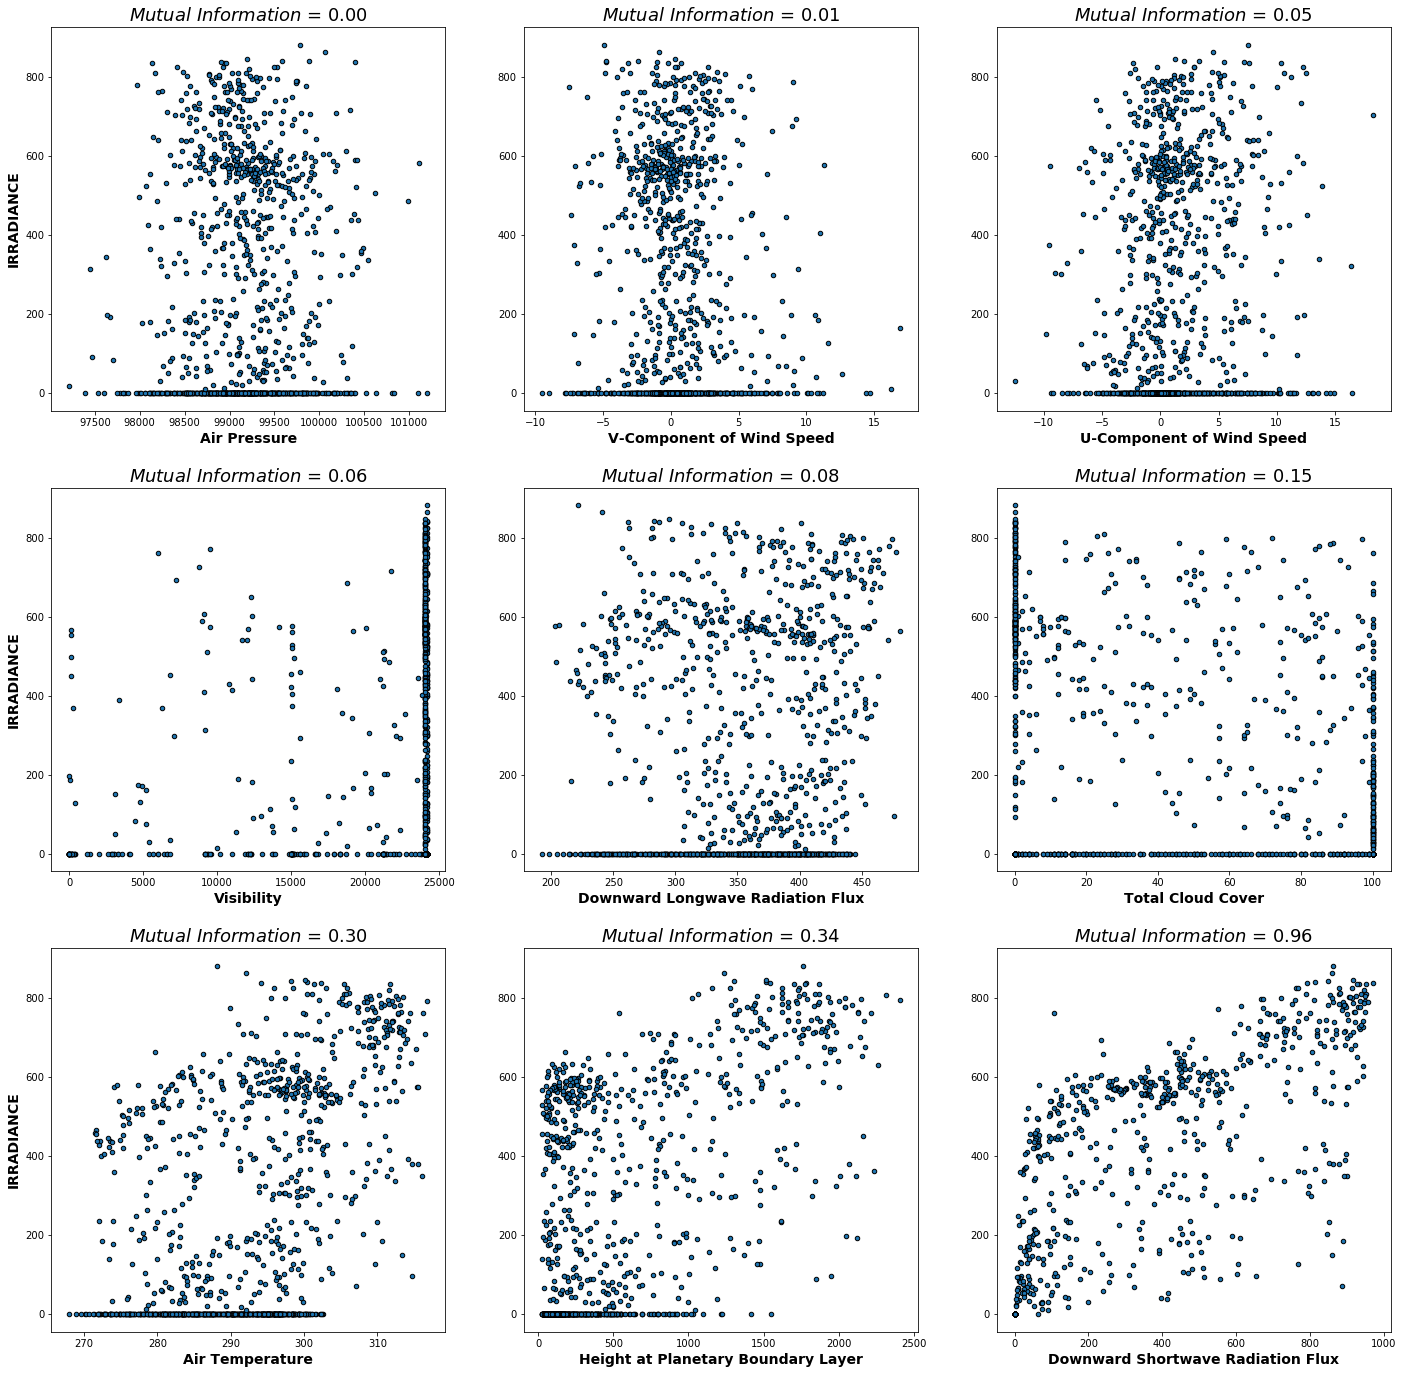
\includegraphics[width=\textwidth]{chapter3/fig_mi_ugabpoa1irr.png}
    	\caption[Mutual information between different NAM weather parameter projections and corresponding solar array B irradiance observations.]{Mutual information between feature projections of different weather parameters in NAM Forecast Model, and the corresponding solar array B irradiance observations.}
    	\label{fig:fig_mi_forecast_target_hr1}
    \end{center}
\end{figure}

\par Downward shortwave radiation flux is the total amount of shortwave radiation that reaches the earth's surface, and is a major component of the total solar radiation on the surface of the earth. Thus, it is the most direct parameter in the estimation solar irradiance, and the high mutual importance score between this weather parameter and the irradiance observations from the solar farm can be justified. By absorbing the incoming solar radiation, the Earth warms up, and its temperature rises. As long as the amount of incoming radiative flux is greater than the outgoing radiative flux, the Earth will continue to warm. Thus, the air temperature at the surface is essential in estimating the amount of heat absorbed at that particular location, which in turn reveals information about the amount of solar radiation absorbed by the thermopiles in the pyranometers. 

\par The influence of clouds on solar irradiance is significant. In the absence of visible clouds, aerosols, precipitable water and other atmospheric conditions affect the transmission of solar radiation through atmosphere. In cloudy conditions though, the clouds absorb a significant amount of the shortwave radiation, making parameters like total cloud cover, which is the fraction of the sky covered by visible clouds essential. The planetary boundary layer (PBL) is the lowest part of the atmosphere which is directly influenced by its contact with the planetary surface. The structure of turbulence within this layer is mainly governed by the PBL height, which is higher during the day, and lower and more stable during nighttime \cite{feature_selection_pbl1}. PBL height characterizes the planetary boundary layer in a fairly integrated manner and affects the weather parameters such as cloud cover and heat flux \cite{feature_selection_pbl2}. This makes PBL height an important parameter in predicting solar irradiance.

\par For the machine learning models to be able to capture and reconstruct the underlying relationship between input-output data pairs effectively, input selection is essential. By removing the redundant and misleading data, input selection often helps in reducing the computational costs and improves the accuracy. Several approaches have been defined in literature for the purpose of input selection, but the most popular technique used for this purpose includes using machine learning models such as the random forests which provide in-built feature selection.

\par Random forests perform a built-in feature selection, because the tree-based strategies used by them naturally rank inputs based on how well they improve the purity of the node. They are an ensemble learning technique constructed over a variety of randomized decision trees, each of which is built over a random extraction of features and data observations. The training of these randomized decision trees is done so that the Gini Impurity is decreased, and those features are selected which help decrease this measure \cite{feature_selection_rf}. Thus, random forests help determine the importance of the features in this manner. It was observed that the weather parameters with higher mutual information scores also received high feature importance scores through this technique, thus validating the dependence of the target irradiance observations on this set of parameters.

\par From among the weather parameters, downward shortwave radiation flux (DSWRF\_SFC), synonymous with global horizontal irradiance (GHI) has the maximum dependency on the target irradiance observations from all the three arrays. In \cite{thesis_zach}, Jones et al. used all 36 feature projections at one-hour temporal resolution for each of the environmental attributes, as the predictor variables for machine learning models. In this work, a forecast horizon of 24 hours was selected, and the relationship between the feature projections in this forecast horizon and the irradiance observations corresponding to the target hours in this forecast horizon was studied. 

\begin{figure}[htb]
    \begin{center}
    	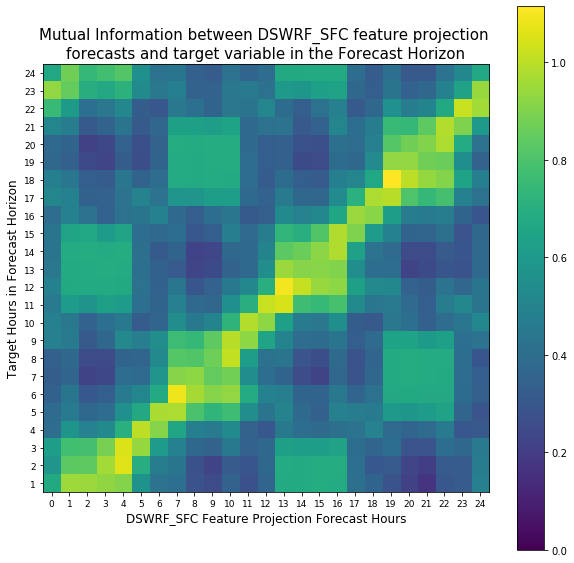
\includegraphics[width=0.65\textwidth]{chapter3/fig_mi_forecast_target.png}
    	\caption[Mutual information between Downward Shortwave Radiation Flux feature projection forecasts and irradiance observations for target hours in the forecast horizon from Solar Array B]{Mutual information between feature projection forecasts of Downward Shortwave Radiation Flux (DSWRF\_SFC) and irradiance observations for target hours in the forecast horizon on Solar Array B.}
    	\label{fig:fig_mi_forecast_target}
    \end{center}
\end{figure}

\par As shown in Fig.~\ref{fig:fig_mi_forecast_target}, it can be observed that the irradiance observations from solar array B for a particular target hour are dependent on only a certain number of feature projections in the forecast horizon. Thus, for each target hour, feature projections from 6 hours ahead, and 6 hours prior were used as predictors. For the first six target hours in the forecast horizon which do not necessarily have six prior feature projections, desired number of feature projections were selected from the end. Similarly, for the last six target hours in the forecast horizon which do not necessarily have six subsequent feature projections, desired number of feature projections were selected from the beginning of the forecast horizon. Such a feature projection selection is justified because it is more likely for the same reference time in two consecutive days to have similar weather conditions. Thus, following this input selections scheme, the NAM model data contributes 13 feature projections for each of the four environmental attributes described earlier, eight temporal features (four for the reference time of the observation, four for the target hour offset from the reference time) towards the post-processing of solar irradiance from each of the solar arrays A, B and E using machine learning models.

\subchapter{Experiment Setup}
\par In this chapter, three series of experiments are performed towards predicting solar irradiance on each of the solar arrays A, B and E. Firstly, solar irradiance forecasting using Numerical Weather Prediction (NWP) models such as North America Mesoscale (NAM) Forecast Model is investigated, replicating the modeling methodology employed in \cite{thesis_zach}. This is compared with the processed NAM dataset obtained, by incorporating the input selection technique described in 3.2. Secondly, a multi-model blending approach is explored, combining the irradiance metrics from NAM Forecast Model and formulations such as Clear-Sky Scaling and Liu-Jordan model in PVLIB. Thirdly, the effect of the spatial expansion of forecast coverage is investigated, by including the weather parameters from a grid of cells around the grid representing Athens. Each of these methodologies are explained in finer detail.

\subsubchapter{Irradiance Forecasting with NAM Weather Forecast Model}
\par In \cite{thesis_zach}, Jones et al. used a variety of machine learning techniques to determine their usefulness in predicting solar irradiance. In the manner described in Section 3.2, North America Mesoscale (NAM) weather forecast data and solar irradiance data from the solar farm at the University of Georgia were collected for the years 2017 and 2018. Planar surface features from the North America Mesoscale (NAM) weather forecast model such as air pressure, geopotential height, height at planetary boundary layer, air temperature, u-component of wind speed, v-component of wind speed, downward shortwave radiation flux and downward longwave radiation flux were used for the purpose of forecasting solar irradiance, 24 hours into the future. The first 36 feature projections of the weather parameters which are at a one-hour temporal resolution were included as the predictor variables for the machine learning models. Additionally, temporal features were considered as well. Models were trained on the data collected during 2017 and evaluated against data collected during 2018.

\par For all machine learning models, finding the ideal set of parameters which define the model architecture, referred to as hyperparameters is paramount. Jones et al performed hyperparameter tuning by carrying out a cross-validated grid search over a parameter space defined around the default hyperparameters given in the \textit{scikit-learn} documentation. The results generated by using these hyperparameters were replicated for the grid representing the NAM forecasts. Following the input selection techniques described in Section 3.2, a new series of machine learning models were trained on the processed NAM dataset. Select feature projections for weather parameters from NAM data such as air temperature, total cloud cover, height at planetary boundary layer and downward shortwave radiation flux were used as predictors for the models, depending on the target hour offset in the forecast horizon. A new set of hyperparameters were picked for these models by performing a randomized cross-validated grid search. These models were trained on data collected during 2017 as well, and evaluated against data collected during 2018. The results obtained by both the methodologies, with and without input selection, were compared and analyzed.

\subsubchapter{Multi-Model Blending Approach }
\par Downward shortwave radiation flux (synonymous with global horizontal irradiance, GHI) was identified to be the most important NAM Weather Forecast Model parameter for solar irradiance forecasting. However, the need to correct the bias in the estimation of this parameter was identified. Irradiance metrics such as global horizontal irradiance (GHI), direct normal irradiance (DNI) and diffuse horizontal irradiance (DHI) can be estimated with the help of several formulations defined in literature. Through the PVLib Forecast Modelling techniques such as Clear-Sky Scaling and Liu-Jordan model, these metrics were estimated from the weather parameters in the NAM data.

\begin{figure}[ht]
    \begin{center}
    	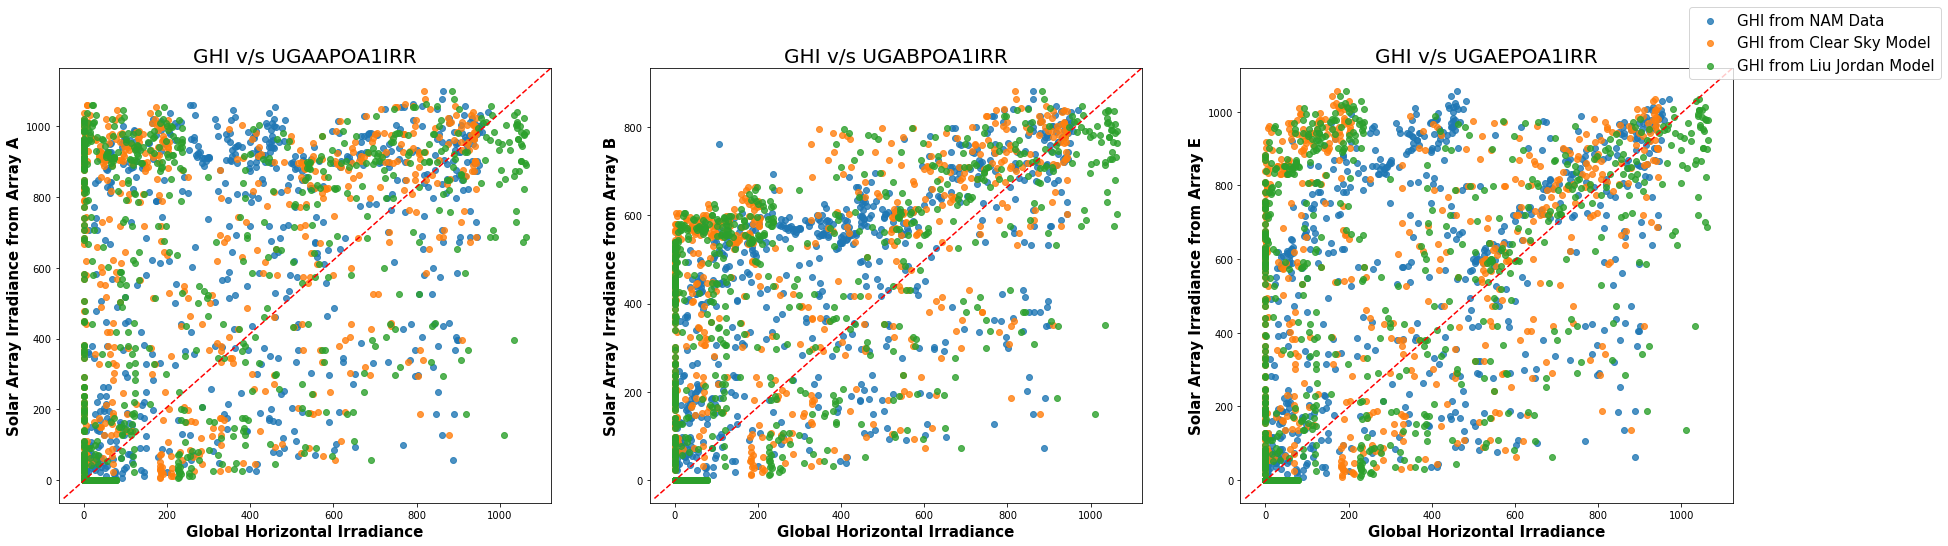
\includegraphics[width=\textwidth]{chapter3/fig_ghi_irradiance.png}
    	\caption[Global horizontal irradiance from NAM data, Clear-sky Scaling and Liu-Jordan against irradiance observations from arrays A, B and E through 2017.]{Global horizontal irradiance from NAM data, Clear-sky Scaling and Liu-Jordan Model against irradiance observations from dual-axis array A (left), fixed-axis array B (center) and single-axis array E (right) through 2017.}
    	\label{fig:fig_ghi_irradiance}
    \end{center}
\end{figure}

\par In this section, a multi-model blending approach is explored, where the weather forecast parameters from NAM are integrated with the irradiance metrics retrieved from Clear-Sky Scaling technique and Liu-Jordan model. Primarily, techniques are explored to combine the GHI parameter from each of the models. In Fig. \ref{fig:fig_ghi_irradiance}, the GHI parameter estimations from each of the models are plotted against the solar irradiance observations from solar arrays A, B and E in the solar farm. 

\subsubsection*{NAM Forecast Model and Clear-Sky Scaling Technique}
The clear-sky scaling technique in \textit{pvlib-python} helps estimate the global horizontal irradiance in clear-sky conditions on the basis of the total cloud cover. Metrics such as clear-sky index help in the removal of diurnal and seasonal signals from a given set of radiation data \cite{expt_clearsky_index}. The clear-sky index for a photovoltaic system can be defined as:\\
\begin{center}
    $K\textsubscript{t} = \frac{GHI\textsubscript{MEAS}}{GHI\textsubscript{CS}}$
\end{center}
where $GHI\textsubscript{MEAS}$ refers to the global horizontal irradiance from a system (which in this case would be $GHI\textsubscript{NAM}$, i.e, global horizontal irradiance from NAM model) and $GHI\textsubscript{CS}$ refers to the global horizontal irradiance from a simulated clear-sky model. The clear-sky index was formulated such that the negative and non-finite values are truncated to zero, and the maximum value is 2, allowing the over-irradiance events typically seen in sub-hourly data.

\begin{figure}[htbp]
    \begin{center}
    	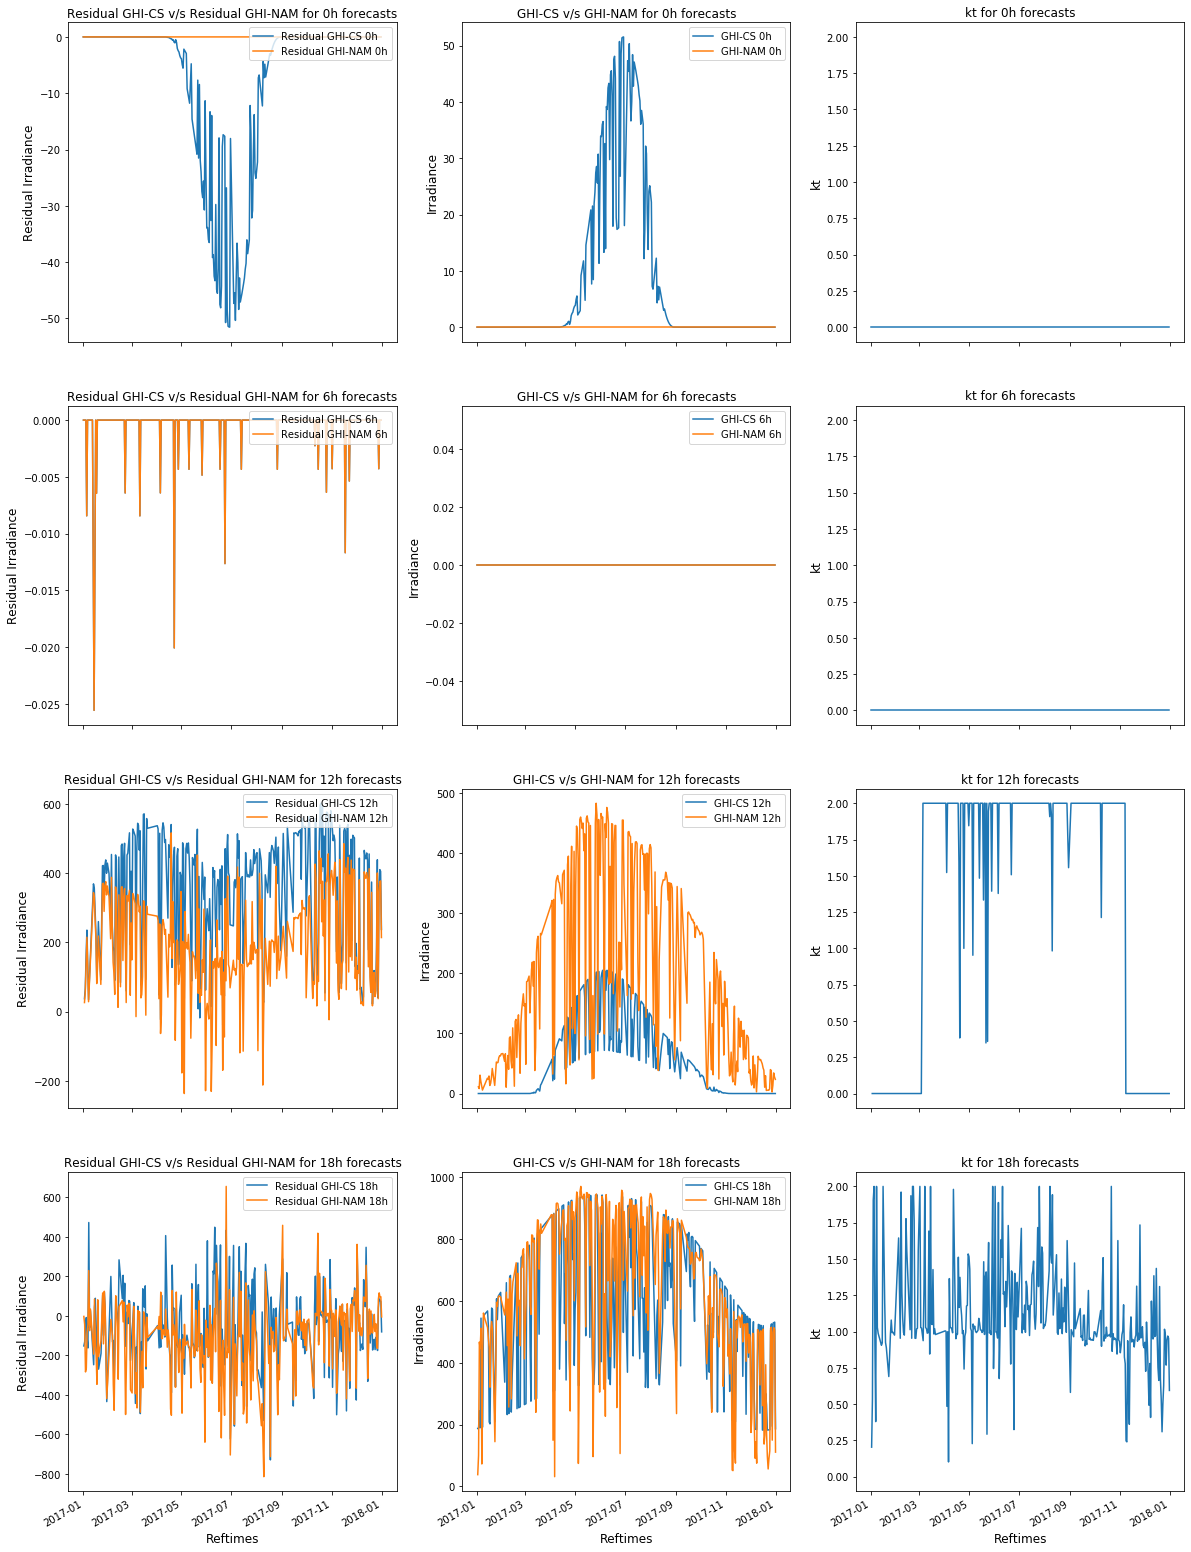
\includegraphics[width=\textwidth]{chapter3/fig_ghi_comparison.png}
    	\caption[Comparing GHI from Clearsky-Scaling ($GHI_{CS}$) and GHI from NAM Forecast Model ($GHI_{NAM}$) for 00h, 06h, 12h, 18h forecasts in 2017]{Comparing GHI from Clearsky-Scaling ($GHI_{CS}$) and GHI from NAM Forecast Model ($GHI_{NAM}$) for 00h, 06h, 12h, 18h forecasts: Residuals of $GHI_{CS}$ and $GHI_{NAM}$ with respect to Array B irradiance observations (left); Clear-sky index ($K_t$) estimations for individual forecasts in 2017 (right).}
    	\label{fig:fig_ghi_comparison}
    \end{center}
\end{figure}

\par In order to assess the $GHI$ values from both NAM model and Clear-Sky Scaling model, residuals between the irradiance observations from solar array B and both $GHI\textsubscript{NAM}$ and $GHI\textsubscript{CS}$ were estimated for the year 2017. Among these, the residuals corresponding to the 00h, 06h, 12h and 18h UTC forecasts were separated, and were plotted in Fig.~\ref{fig:fig_ghi_comparison} (left). The clear-sky index was evaluated for each of the forecasts, and corresponding plots were drawn in Fig.~\ref{fig:fig_ghi_comparison} (right). It was observed that the clear-sky index was constantly zero for the 00h and 06h forecasts throughout the year. This can be attributed to the fact that these forecasts correspond to the time of darkness, resulting in no solar radiation being captured in the solar arrays. Additionally, it can be seen that the residuals for $GHI\textsubscript{NAM}$ are consistently better than the $GHI\textsubscript{CS}$ values for the 12h forecasts, while for the 18h forecasts, they are inconclusive. Thus, the 12h and 18h forecasts were further analyzed with respect to the clear-sky index values.

\begin{table}[h]
\begin{center}
    \caption{MAE of $GHI_{CS}$ and $GHI_{NAM}$ with Array B irradiance for 12h and 18h forecasts.}
    \label{Tab:mean_absolute_residual}
    \begin{tabular}{ c c c c }
    	\toprule
    	\textbf{\parbox{2cm}{\centering Forecast Hour}} & \boldmath\textbf{$K_t$} & \textbf{\parbox{4.5cm}{\centering Mean Absolute Error of \boldmath$GHI_{CS}$}} & \textbf{\parbox{4.5cm}{\centering Mean Absolute Error of \boldmath$GHI_{NAM}$}}\\
    	\midrule
    	\multirow{3}{4em}{$12$} & $< 1.5$ & 271.003 & 219.064 \\ &
    	$> 1.5$ & 383.122 & 204.682 \\
    	\midrule
    	\multirow{3}{4em}{$18$} & $< 1.5$ & 155.63 & 157.38 \\ &
    	$> 1.5$ & 172.869 & 229.998 \\
    	\bottomrule
    \end{tabular}
\end{center}
\end{table}

\par In Table \ref{Tab:mean_absolute_residual}, mean of the absolute values of the residuals (MAE) was computed for the 12h and 18h forecasts, depending on the clear-sky index values estimated for the forecasts. It was observed that for the 12h forecasts, irrespective of $K_t$, $MAD$ corresponding to $GHI_{NAM}$ was lower than that of $GHI_{CS}$, indicating that the GHI predicted by NAM for these forecasts were a better estimation. However, for the 18h forecasts, $MAD$ for forecasts with $K_t < 1.5$ was marginally better for $GHI_{CS}$. Additionally, the $MAD$ for 18h forecasts with $K_t > 1.5$ was significantly better for $GHI_{CS}$, as compared to $GHI_{NAM}$. Thus, it can be concluded that the NAM model tends to overpredict GHI in clear-sky conditions. Thus, in order to correct this bias, for all the 18h forecasts with a $K_t$ value greater than 1.5, $GHI\textsubscript{NAM}$ and $GHI\textsubscript{CS}$ are averaged.

\par From the Clearsky Scaling technique in \textit{pvlib-python}, three irradiance metrics, i.e, GHI, DHI and DNI are retrieved. GHI, which is calculated by scaling total cloud cover, and DNI, which is calculated from the DISC method are highly correlated. Also, DHI, which is empirically calculated from both GHI and DNI, is highly correlated with GHI. Thus, to avoid multicollinearity, the remaining two irradiance metrics, i.e, DHI and DNI are not considered as explanatory variables for the post-processing of irradiance using machine learning models, resulting in the use of only GHI ($GHI_{CS}$) to correct the bias in GHI estimations in NAM model ($GHI_{NAM})$.

\subsubsection*{NAM Forecast Model and Liu-Jordan Model}

The Liu-Jordan Model in \textit{pvlib-python} helps estimate the three irradiance metrics as well. Additionally, this model has been shown to be effective in predicting diffuse irradiance on inclined surfaces. Thus, it was hypothesized that this parameter would help improving irradiance forecasting on solar array A (dual-axis tracking array) and solar array E (single-axis tracking array), which move along their axes based on the position of the sun. In this model, DNI is estimated from transmittance, DHI based on transmittance and solar zenith angle, and GHI is empirically formulated from DHI and DNI. Additionally, it was observed that the GHI observations through this formulation for the year 2017 are highly correlated with DNI. Thus, to avoid multicollinearity amongst the estimators, only GHI and DHI are included along with the estimators from the NAM model for the post-processing of solar irradiance using machine learning models.

\subsubchapter{Geographic Expansion of Forecast Coverage}
Lorenz et al. \cite{expansion_lorenz} found that expanding the forecast region to approximately $100 km$ x $100 km$ and performing a spatial averaging across the region resulted in an improvement in day-ahead solar forecasting. Sanders et. al. \cite{publication_sanders} and Jones et al. \cite{thesis_zach} showed that including the weather forecasts from the grids around the Athens grid resulted in an improved day-ahead solar forecasting as well, though the latter observed that the improvement diminishes as the grid-size grows larger. Additionally, Jones et al also noted that a $3$ x $3$ grid of NAM forecasts centered around Athens, GA, equivalent to a $36km$ x $36km$ area was optimal. A similar geographic expansion of forecast coverage was performed with $3$ x $3$ and $5$ x $5$ grid of NAM forecasts around Athens, GA, resulting in a spatial expansion upto $60km$ x $60km$. The dataset set up using the multi-model blending approach described in 3.3.2, was used to determine the effect of geographic expansion.

\begin{figure}[ht]
    \begin{center}
    	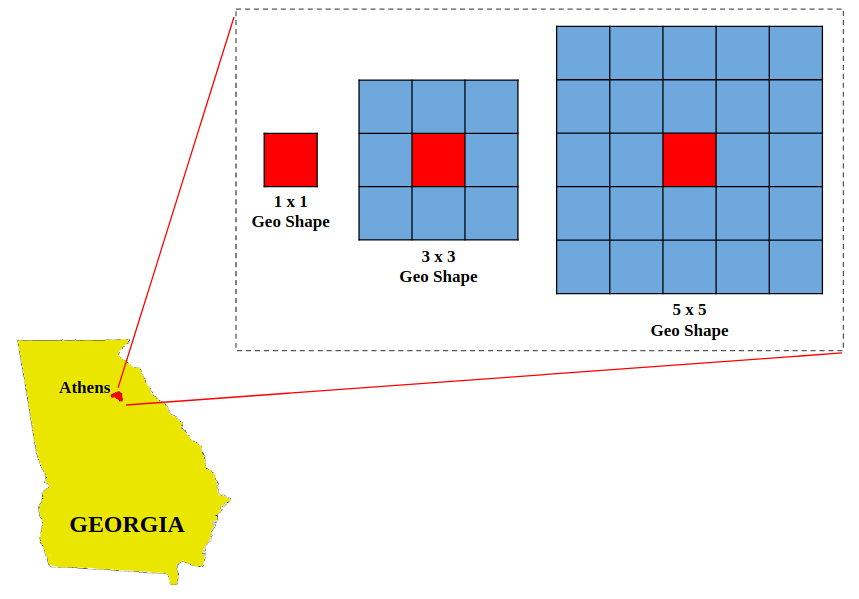
\includegraphics[width=0.65\textwidth]{chapter3/fig_geoshapes.png}
    	\caption[Geographic expansion of forecast coverage around Athens NAM model data grid]{Geographic expansion of forecast coverage with 1 x 1 Geo Shape representing Athens NAM model data grid, 3 x 3 Geo Shape and 5 x 5 Geo Shape representing grid of cells around Athens.}
    	\label{fig:fig_geoshapes}
    \end{center}
\end{figure}

\subchapter{Results and Discussion}
\par In \cite{thesis_zach}, Jones et al used a 24-hour \textit{persistence model} to set a baseline for the more sophisticated machine learning models. In general, persistence models are based on the assumption that conditions remain unchanged between the current time and a future time. The 24-hour persistence models would measure the solar irradiance at a particular time $t$ based on the irradiance value measured at $t-24$. Making use of such a trivial model as a baseline helps in understanding and preparing the data better, by providing a reference for improving the model. Similar 24-hour \textit{persistence models} were used as a baseline in this work as well.

\par Several machine learning algorithms such as least-squares linear regression (LSLR), k-Nearest Neighbors (KNN), Support Vector Regression (SVR), Decision Trees (DT), Random Forests (RF) and Extreme Gradient Boosted Trees (XGBT) were used for the purpose of forecasting. Weather parameter inputs from the NAM data were used as inputs to the machine learning models, and the irradiance observations from the solar arrays A, B and E were used as the target variables. Prediction of target irradiance was done for a forecast horizon of 24 hours, i.e, solar irradiance on each of the arrays was predicted 24 hours into the future, at a one hour temporal resolution. Models were trained on data collected during 2017, and evaluated against data collected during 2018. The performance of the machine learning models were evaluated based on the metrics such as \textit{mean absolute error (MAE)} and $R^2$.  

\par Separate machine learning models were trained for each of the target hour offsets between 1 and 24, and their results were analyzed in two schemes: mean of the evaluations for each forecast hour in the forecast horizon ($Overall$); mean of the evaluations for sets of six forecast hours in the forecast horizon, i.e, $1 - 6$, $7 - 12$, $13 - 18$ and $19 - 24$. Such an analysis helped in realizing the performance of the models specifically for different periods in the day. 

\par In this work, an input selection scheme as described in 3.2 was incorporated towards selecting features for the machine learning models. As a part of this scheme, the key differences between Jones' dataset and the one used in this work, towards training with the machine learning models are as follows: Jones et al hadn't considered the \textit{total cloud cover} parameter in the NAM weather dataset; from among the other surface weather variables used, only air temperature, height at planetary boundary layer and downward shortwave radiation flux were considered; instead of the 36 feature projections for each of the weather variables, select feature projections depending on the target hour offset were chosen; design of the temporal features was different. Based on these differences, the two NAM datasets were used as input to different machine learning models.


\begin{table}[h]
\begin{center}
    \caption{Evaluating performance of machine learning algorithms trained against solar array A using NAM Forecast Model data, with and without input selection.}
    \vspace{0.2cm}
    \label{Tab:fs_array_a}
    \begin{tabular}{@{}p{5.3em}ccccccccc@{}}
    \toprule
    \textbf{Methodology} & \textbf{Metric} & \textbf{Horizon} & \textbf{PER} & \textbf{LSLR} & \textbf{SVR} & \textbf{KNN} & \textbf{DT} & \textbf{RF} & \textbf{XGBT} \\ \cmidrule(l){1-10} 
    \multirow{10}{5em}{Without Input Selection} & \multirow{5}{*}{$MAE$} & $1 - 6$ & \_\_ & \_\_ & \_\_ & \_\_ & \_\_ & \_\_ & \_\_ \\
                                              &                   & $7 - 12$ & \_\_ & \_\_ & \_\_ & \_\_ & \_\_ & \_\_ & \_\_ \\
                                              &                   & $13 - 18$ & \_\_ & \_\_ & \_\_ & \_\_ & \_\_ & \_\_ & \_\_ \\
                                              &                   & $19 - 24$ & \_\_ & \_\_ & \_\_ & \_\_ & \_\_ & \_\_ & \_\_ \\
                                              &                   & $Overall$ & \_\_ & \_\_ & \_\_ & \_\_ & \_\_ & \_\_ & \_\_ \\ \cmidrule(lr){2-10}
                                              & \multirow{5}{*}{$R^2$} & $1 - 6$ & \_\_ & \_\_ & \_\_ & \_\_ & \_\_ & \_\_ & \_\_ \\
                                              &                   & $7 - 12$ & \_\_ & \_\_ & \_\_ & \_\_ & \_\_ & \_\_ & \_\_ \\
                                              &                   & $13 - 18$ & \_\_ & \_\_ & \_\_ & \_\_ & \_\_ & \_\_ & \_\_ \\
                                              &                   & $19 - 24$ & \_\_ & \_\_ & \_\_ & \_\_ & \_\_ & \_\_ & \_\_ \\
                                              &                   & $Overall$ & \_\_ & \_\_ & \_\_ & \_\_ & \_\_ & \_\_ & \_\_ \\ 
    \midrule
    Relative Imp. & $\bigtriangleup MAE$ (\%)  & $Overall$ & $-$ & \_\_ & \_\_ & \_\_ & \_\_ & \_\_ & \_\_ \\ 
    \midrule
    \multirow{10}{5em}{Input Selection}
                                              & \multirow{5}{*}{$MAE$} & $1 - 6$ & \_\_ & \_\_ & \_\_ & \_\_ & \_\_ & \_\_ & \_\_ \\
                                              &                   & $6 - 12$ & \_\_ & \_\_ & \_\_ & \_\_ & \_\_ & \_\_ & \_\_ \\
                                              &                   & $13 - 18$ & \_\_ & \_\_ & \_\_ & \_\_ & \_\_ & \_\_ & \_\_ \\
                                              &                   & $19 - 24$ & \_\_ & \_\_ & \_\_ & \_\_ & \_\_ & \_\_ & \_\_ \\
                                              &                   & $Overall$ & \_\_ & \_\_ & \_\_ & \_\_ & \_\_ & \_\_ & \_\_ \\ \cmidrule(lr){2-10}
                                              & \multirow{5}{*}{$R^2$} & $1 - 6$ & \_\_ & \_\_ & \_\_ & \_\_ & \_\_ & \_\_ & \_\_ \\
                                              &                   & $7 - 12$ & \_\_ & \_\_ & \_\_ & \_\_ & \_\_ & \_\_ & \_\_ \\
                                              &                   & $13 - 18$ & \_\_ & \_\_ & \_\_ & \_\_ & \_\_ & \_\_ & \_\_ \\
                                              &                   & $19 - 24$ & \_\_ & \_\_ & \_\_ & \_\_ & \_\_ & \_\_ & \_\_ \\
                                              &                   & $Overall$ & \_\_ & \_\_ & \_\_ & \_\_ & \_\_ & \_\_ & \_\_ \\ 
    \bottomrule
    \end{tabular}
\end{center}
\end{table}

\begin{table}[h]
\begin{center}
    \caption{Evaluating performance of machine learning algorithms trained against solar array B using NAM Forecast Model data, with and without input selection.}
    \vspace{0.2cm}
    \begin{tabular}{@{}p{5.3em}ccccccccc@{}}
    \toprule
    \textbf{Methodology} & \textbf{Metric} & \textbf{Horizon} & \textbf{PER} & \textbf{LSLR} & \textbf{SVR} & \textbf{KNN} & \textbf{DT} & \textbf{RF} & \textbf{XGBT} \\ \cmidrule(l){1-10} 
    \multirow{10}{5em}{Without Input Selection} & \multirow{5}{*}{$MAE$} & $1 - 6$ & \_\_ & \_\_ & \_\_ & \_\_ & \_\_ & \_\_ & \_\_ \\
                                              &                   & $7 - 12$ & \_\_ & \_\_ & \_\_ & \_\_ & \_\_ & \_\_ & \_\_ \\
                                              &                   & $13 - 18$ & \_\_ & \_\_ & \_\_ & \_\_ & \_\_ & \_\_ & \_\_ \\
                                              &                   & $19 - 24$ & \_\_ & \_\_ & \_\_ & \_\_ & \_\_ & \_\_ & \_\_ \\
                                              &                   & $Overall$ & \_\_ & \_\_ & \_\_ & \_\_ & \_\_ & \_\_ & \_\_ \\ \cmidrule(lr){2-10}
                                              & \multirow{5}{*}{$R^2$} & $1 - 6$ & \_\_ & \_\_ & \_\_ & \_\_ & \_\_ & \_\_ & \_\_ \\
                                              &                   & $7 - 12$ & \_\_ & \_\_ & \_\_ & \_\_ & \_\_ & \_\_ & \_\_ \\
                                              &                   & $13 - 18$ & \_\_ & \_\_ & \_\_ & \_\_ & \_\_ & \_\_ & \_\_ \\
                                              &                   & $19 - 24$ & \_\_ & \_\_ & \_\_ & \_\_ & \_\_ & \_\_ & \_\_ \\
                                              &                   & $Overall$ & \_\_ & \_\_ & \_\_ & \_\_ & \_\_ & \_\_ & \_\_ \\ 
    \midrule
    Relative Imp. & $\bigtriangleup MAE$ (\%)  & $Overall$ & $-$ & \_\_ & \_\_ & \_\_ & \_\_ & \_\_ & \_\_ \\ 
    \midrule
    \multirow{10}{5em}{Input Selection}
                                              & \multirow{5}{*}{$MAE$} & $1 - 6$ & \_\_ & \_\_ & \_\_ & \_\_ & \_\_ & \_\_ & \_\_ \\
                                              &                   & $6 - 12$ & \_\_ & \_\_ & \_\_ & \_\_ & \_\_ & \_\_ & \_\_ \\
                                              &                   & $13 - 18$ & \_\_ & \_\_ & \_\_ & \_\_ & \_\_ & \_\_ & \_\_ \\
                                              &                   & $19 - 24$ & \_\_ & \_\_ & \_\_ & \_\_ & \_\_ & \_\_ & \_\_ \\
                                              &                   & $Overall$ & \_\_ & \_\_ & \_\_ & \_\_ & \_\_ & \_\_ & \_\_ \\ \cmidrule(lr){2-10}
                                              & \multirow{5}{*}{$R^2$} & $1 - 6$ & \_\_ & \_\_ & \_\_ & \_\_ & \_\_ & \_\_ & \_\_ \\
                                              &                   & $7 - 12$ & \_\_ & \_\_ & \_\_ & \_\_ & \_\_ & \_\_ & \_\_ \\
                                              &                   & $13 - 18$ & \_\_ & \_\_ & \_\_ & \_\_ & \_\_ & \_\_ & \_\_ \\
                                              &                   & $19 - 24$ & \_\_ & \_\_ & \_\_ & \_\_ & \_\_ & \_\_ & \_\_ \\
                                              &                   & $Overall$ & \_\_ & \_\_ & \_\_ & \_\_ & \_\_ & \_\_ & \_\_ \\ 
    \bottomrule
    \end{tabular}
\end{center}
\end{table}

\begin{table}[h]
\begin{center}
    \caption{Evaluating performance of machine learning algorithms trained against solar array E using NAM Forecast Model data, with and without input selection.}
    \vspace{0.2cm}
    \begin{tabular}{@{}p{5.3em}ccccccccc@{}}
    \toprule
    \textbf{Methodology} & \textbf{Metric} & \textbf{Horizon} & \textbf{PER} & \textbf{LSLR} & \textbf{SVR} & \textbf{KNN} & \textbf{DT} & \textbf{RF} & \textbf{XGBT} \\ \cmidrule(l){1-10} 
    \multirow{10}{5em}{Without Input Selection} & \multirow{5}{*}{$MAE$} & $1 - 6$ & \_\_ & \_\_ & \_\_ & \_\_ & \_\_ & \_\_ & \_\_ \\
                                              &                   & $7 - 12$ & \_\_ & \_\_ & \_\_ & \_\_ & \_\_ & \_\_ & \_\_ \\
                                              &                   & $13 - 18$ & \_\_ & \_\_ & \_\_ & \_\_ & \_\_ & \_\_ & \_\_ \\
                                              &                   & $19 - 24$ & \_\_ & \_\_ & \_\_ & \_\_ & \_\_ & \_\_ & \_\_ \\
                                              &                   & $Overall$ & \_\_ & \_\_ & \_\_ & \_\_ & \_\_ & \_\_ & \_\_ \\ \cmidrule(lr){2-10}
                                              & \multirow{5}{*}{$R^2$} & $1 - 6$ & \_\_ & \_\_ & \_\_ & \_\_ & \_\_ & \_\_ & \_\_ \\
                                              &                   & $7 - 12$ & \_\_ & \_\_ & \_\_ & \_\_ & \_\_ & \_\_ & \_\_ \\
                                              &                   & $13 - 18$ & \_\_ & \_\_ & \_\_ & \_\_ & \_\_ & \_\_ & \_\_ \\
                                              &                   & $19 - 24$ & \_\_ & \_\_ & \_\_ & \_\_ & \_\_ & \_\_ & \_\_ \\
                                              &                   & $Overall$ & \_\_ & \_\_ & \_\_ & \_\_ & \_\_ & \_\_ & \_\_ \\ 
    \midrule
    Relative Imp. & $\bigtriangleup MAE$ (\%)  & $Overall$ & $-$ & \_\_ & \_\_ & \_\_ & \_\_ & \_\_ & \_\_ \\ 
    \midrule
    \multirow{10}{5em}{Input Selection}
                                              & \multirow{5}{*}{$MAE$} & $1 - 6$ & \_\_ & \_\_ & \_\_ & \_\_ & \_\_ & \_\_ & \_\_ \\
                                              &                   & $6 - 12$ & \_\_ & \_\_ & \_\_ & \_\_ & \_\_ & \_\_ & \_\_ \\
                                              &                   & $13 - 18$ & \_\_ & \_\_ & \_\_ & \_\_ & \_\_ & \_\_ & \_\_ \\
                                              &                   & $19 - 24$ & \_\_ & \_\_ & \_\_ & \_\_ & \_\_ & \_\_ & \_\_ \\
                                              &                   & $Overall$ & \_\_ & \_\_ & \_\_ & \_\_ & \_\_ & \_\_ & \_\_ \\ \cmidrule(lr){2-10}
                                              & \multirow{5}{*}{$R^2$} & $1 - 6$ & \_\_ & \_\_ & \_\_ & \_\_ & \_\_ & \_\_ & \_\_ \\
                                              &                   & $7 - 12$ & \_\_ & \_\_ & \_\_ & \_\_ & \_\_ & \_\_ & \_\_ \\
                                              &                   & $13 - 18$ & \_\_ & \_\_ & \_\_ & \_\_ & \_\_ & \_\_ & \_\_ \\
                                              &                   & $19 - 24$ & \_\_ & \_\_ & \_\_ & \_\_ & \_\_ & \_\_ & \_\_ \\
                                              &                   & $Overall$ & \_\_ & \_\_ & \_\_ & \_\_ & \_\_ & \_\_ & \_\_ \\ 
    \bottomrule
    \end{tabular}
\end{center}
\end{table}


\begin{table}[h]
\begin{center}
    \caption{Sample Table 1}
    \begin{tabular}{ c c c c c c c c c}
    	\toprule
    	\textbf{Metric} & \textbf{Horizon} & \textbf{PER} & \textbf{LSLR} & \textbf{SVR} & \textbf{KNN} & \textbf{DT} & \textbf{RF} & \textbf{XGBT}\\
    	\midrule
    	\multirow{3}{4em}{$MAE$} & $1 - 6$ & \_\_ & \_\_ & \_\_ & \_\_ & \_\_ & \_\_ & \_\_\\ &
    	$7 - 12$ & \_\_ & \_\_ & \_\_ & \_\_ & \_\_ & \_\_ & \_\_\\ &
    	$13 - 18$ & \_\_ & \_\_ & \_\_ & \_\_ & \_\_ & \_\_ & \_\_\\ &
    	$19 - 24$ & \_\_ & \_\_ & \_\_ & \_\_ & \_\_ & \_\_ & \_\_\\ &
    	$Overall$ & \_\_ & \_\_ & \_\_ & \_\_ & \_\_ & \_\_ & \_\_\\
    	\midrule
    	\multirow{3}{4em}{$R^2$} & $1 - 6$ & \_\_ & \_\_ & \_\_ & \_\_ & \_\_ & \_\_ & \_\_ \\ &
    	$7 - 12$ & \_\_ & \_\_ & \_\_ & \_\_ & \_\_ & \_\_ & \_\_\\ &
    	$13 - 18$ & \_\_ & \_\_ & \_\_ & \_\_ & \_\_ & \_\_ & \_\_\\ &
    	$19 - 24$ & \_\_ & \_\_ & \_\_ & \_\_ & \_\_ & \_\_ & \_\_\\ &
    	$Overall$ & \_\_ & \_\_ & \_\_ & \_\_ & \_\_ & \_\_ & \_\_\\
    	\bottomrule
    \end{tabular}
\end{center}
\end{table}

\begin{table}[h]
\begin{center}
    \caption{Sample Table 2}
    \begin{tabular}{l l l l l l l l l l l}
        \toprule
        \multirow{2}{*}{\textbf{Metric}} & \multirow{2}{*}{\textbf{Horizon}} & \multicolumn{3}{c}{\textbf{KNN}} & \multicolumn{3}{c}{\textbf{RF}} & \multicolumn{3}{c}{\textbf{XGBT}}\\
        \cmidrule{3-11}
         &  & 1x1 & 3x3 & 5x5 & 1x1 & 3x3 & 5x5 & 1x1 & 3x3 & 5x5 \\
        \midrule
        \multirow{5}{*}{$MAE$} & $1 - 6$ & \_ & \_ & \_ & \_ & \_ & \_ & \_ & \_ & \_ \\
        & $7 - 12$ & \_ & \_ & \_ & \_ & \_ & \_ & \_ & \_ & \_ \\
        & $13 - 18$ & \_ & \_ & \_ & \_ & \_ & \_ & \_ & \_ & \_ \\
        & $19 - 24$ & \_ & \_ & \_ & \_ & \_ & \_ & \_ & \_ & \_ \\
        & $Overall$ & \_ & \_ & \_ & \_ & \_ & \_ & \_ & \_ & \_ \\
        \midrule
        \multirow{5}{*}{$R^2$} & $1 - 6$ & \_ & \_ & \_ & \_ & \_ & \_ & \_ & \_ & \_ \\
        & $7 - 12$ & \_ & \_ & \_ & \_ & \_ & \_ & \_ & \_ & \_ \\
        & $13 - 18$ & \_ & \_ & \_ & \_ & \_ & \_ & \_ & \_ & \_ \\
        & $19 - 24$ & \_ & \_ & \_ & \_ & \_ & \_ & \_ & \_ & \_ \\
        & $Overall$ & \_ & \_ & \_ & \_ & \_ & \_ & \_ & \_ & \_ \\
        \bottomrule
    \end{tabular}
\end{center}
\end{table}

\newpage